\chapter{Git}
\section{¿Qué es Git?}
Git es es un sistema de control de versiones distribuido que permite a los desarrolladores llevar un registro de los cambios en sus archivos y coordinar el trabajo en proyectos de software de manera eficiente.\\

Distribuido quiere decir que no depende de un único sitio en específico para almacenar su código. Existen muchos controladores de versiones, pero no todos son distribuidos, eso significa que por ejemplo si el servidor donde tienen almacenado el código llega a reventar, entonces perderían todo el código.\\

En cambio, un sistema distribuido permite tener a todos los colaboradores una copia del proyecto en sus propios equipos, y en caso de que el servidor principal reventase, el proyecto seguiría existiendo en las máquinas personales de los desarrolladores y se podría recuperar.

\section{Comandos de Git}

\subsection{Git Init}
Para empezar a usar git, primero se necesita un repositorio local, es decir una carpeta, sobre la cual git va a ir controlando y guardando sus versiones y revisando sus cambios.\\

Una vez creada la carpeta, desde la terminal hay que posicionarse sobre esa carpeta (en bash con cd ~/directorio).\\

Una vez hecho esto en la terminal se va a escribir, \textbf{git init} y esto automáticamente creará una carpeta oculta llamada ".git" en la carpeta.\\
\begin{figure}[h!]
	\centering
	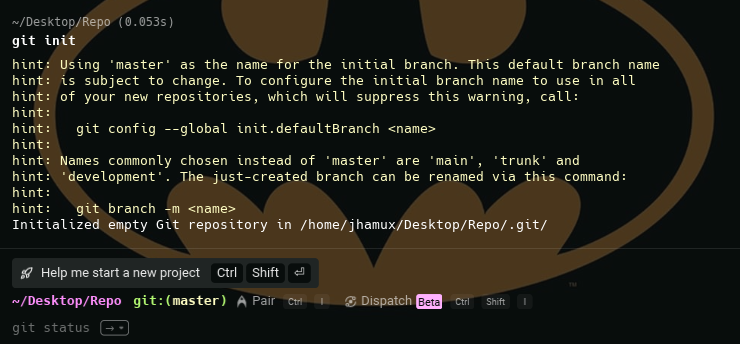
\includegraphics[scale = 0.7]{Images/gitinit}
	\caption{Git Init ejecutado en la terminal}
	
	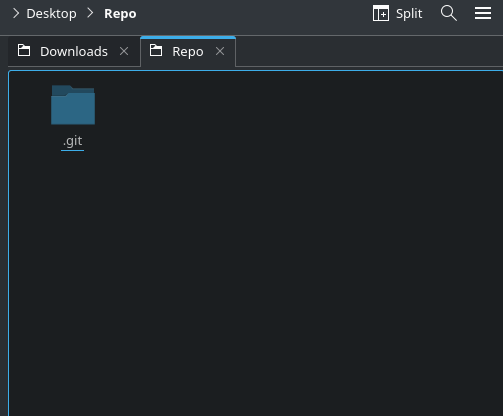
\includegraphics[scale = 0.7]{Images/dotgit}
	\caption{Carpeta Oculta .git en el repositorio}
\end{figure}


Git Init
Git add
Git commit
Git ammend
Git "3 estados"
Git Restore